In this chapter, we introduce the structure of the brain and the principles of dMRI. We then outline key modeling approaches, from traditional DTI to advanced methods such as Multi-Tissue and Local Response Constrained Spherical Deconvolution, which generate orientation distribution functions and enable fixel-based analysis (FBA). Finally, we review applications of DTI and FBA in studying chemobrain in breast cancer patients and present the aim of the thesis.

\section{The Brain}
The brain is an important and complex organ whose functional units are called neurons. Each neuron has a cell body (soma) containing the nucleus, which receives inputs from neighboring neurons through the dendrites. When these inputs reach a certain threshold, the neuron generates an output signal in the axon. The axon is an elongated extension of the neuron that transmits the signal to the connection point with the next neuron or target organs. These points of exchange are called synapses, the junctions where communication takes place. Neurons transmit information through electrical signals called action potentials. As ions move across the cell membrane, the membrane potential changes, triggering similar changes in adjacent regions. This propagates the electrical signal along the neuron. Axons are often surrounded by an insulating layer called myelin, which allows efficient transmission of electrical impulses with minimal loss of signal. Axons typically range from 0.2 to 20 $\mu$m in diameter and are organized into coherent bundles \cite{Edgar2013}. Due to the color imparted by the myelin sheath, these bundles are referred to as white matter. White matter is crucial in connecting different brain regions and transmitting information in the form of electrical signals. It is therefore essential for many brain functions and must be carefully preserved during brain surgery. Numerous neurodegenerative diseases are associated with the disruption or degeneration of axons.

\begin{figure}[h]
  \centering
  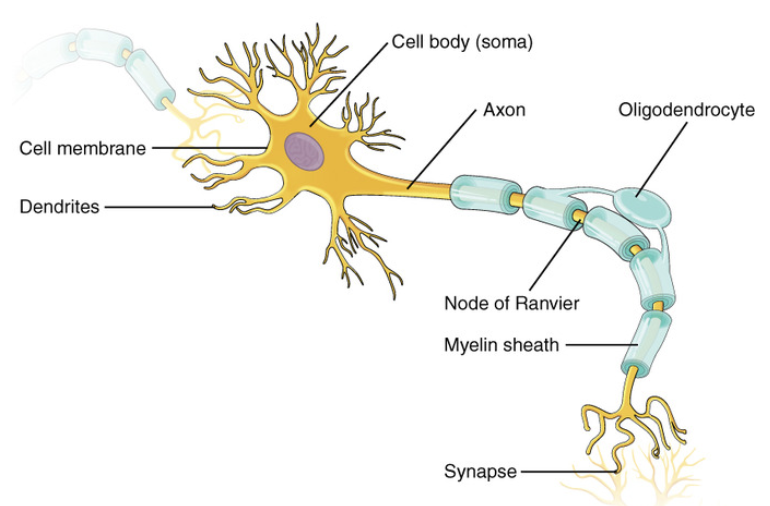
\includegraphics[width=0.7\textwidth]{neuron} % or use height= for vertical sizing
  \caption{Structure of a neuron \cite{Bond2022}.}
  \label{fig:neuron}
\end{figure}

To investigate white matter degeneration, we need tools that can probe the brain's microstructure. For this purpose, the structural characteristics of white matter as a highly organized tissue can be exploited: individual axons contain aligned microtubules, and groups of axons running in the same direction form coherent fibre bundles \cite{Assaf2013}. This makes white matter an ordered and highly directional tissue.

Water is a major component of white matter and exists in both intracellular and extracellular spaces. Water molecules undergo random motion due to thermal energy, a process known as diffusion. In free water, diffusion occurs equally in all directions (isotropic diffusion). However, given the ordered structure of white matter, diffusion becomes anisotropic. Water diffuses more easily along the direction of the axons, while diffusion perpendicular to the axons is hindered by cell membranes and the myelin sheath \cite{Beaulieu2013}. This is different from the surrounding tissues: in gray matter, diffusion is hindered equally in all directions, while in cerebrospinal fluid, it resembles free, isotropic diffusion.
This anisotropic diffusion is a distinctive feature of white matter, that can be exploited using Diffusion-weighted MRI. This non-invasive imaging technique enables the visualization of white matter fibre pathways and provides insights into their structure.

\section{Diffusion-weighted MRI}

 In free diffusion, molecular displacement follows a Gaussian distribution. According to Einstein's equation the mean displacement ($\sigma$=$\sqrt{2Dt}$) increases with both the diffusion coefficient D and the diffusion time t \cite{Mori20143}. In such conditions, the probability of diffusing of a given distance is equal in all directions, so diffusion is isotropic.
In biological tissues, however, water molecules encounter barriers such as cell membranes, which hinder their movement and reduce their diffusion displacement. As a result, the diffusion coefficient is lower than in free water and is referred to as the apparent diffusion coefficient (ADC). The ADC is influenced by the tissue's microscopic structure. In white matter (WM), diffusion is not isotropic: water molecules face more obstacles when moving perpendicular to axonal fibres than when moving along them. This directional dependence means a single diffusion coefficient is insufficient to describe water diffusion in WM and the ADC depends on the measurement direction.

 dMRI enables the investigation of tissue microstructure by measuring water molecule displacements. By quantifying ADC in multiple directions, with dMRI we can infer the orientation of WM fibres. Water molecules thus act as probes, revealing the tissue's microstructure and enabling the mapping of WM tracts, assuming diffusion is greatest along the direction of the fibre bundles \cite{LeBihan2003}. As such, dMRI is a valuable tool for studying WM anatomy and detecting pathological changes.

In MRI, image intensity depends on water concentration (proton density) and signal relaxation times. To make the signal sensitive to water diffusion, a pair of magnetic field gradient pulses can be applied. These gradients have an intensity that varies along a certain direction and are applied for a short period of time, 1-100ms.
When protons are placed in a magnetic field ${\ B}_0$, they acquire a precessing frequency proportional to the field strength, as described by the Larmor equation \cite{Jones2013}: 
\begin{equation}
\omega = \gamma{\ B}_0
\end{equation}

where $\gamma$ is the gyromagnetic ratio (2.7653108 rad/s$\cdot{T}$).
In a dMRI measurement, at first, all protons experience the same ${\ B}_0$, so they have the same frequency and phase. When the first gradient (called dephasing gradient) is applied, the magnetic field becomes position-dependent, causing protons to resonate at slightly different frequencies. In essence, the gradient "labels" the molecules by assigning them frequencies based on their spatial location. Once the gradient is switched off, all protons return to precessing at the same base frequency, but they now possess different phases. After a time $\Delta$, the second gradient (rephasing gradient) is applied. This gradient has the same amplitude and duration as the first one but with the opposite sign (or the same sign in the case of a spin-echo sequence, where a $180^\circ$ refocusing pulse is applied) \cite{Mori20142}.  When this second gradient is turned off, all protons again precess at the same frequency. If a molecule remained at exactly the same position during the interval $\Delta$, the phase shift induced by the first gradient is canceled by the second, and the net phase difference becomes zero.

However, because water molecules diffuse naturally, their positions are likely to change during $\Delta$. As a result, the phase shifts from the two gradients don't fully cancel out. The distribution of molecular displacements governed by the ADC leads to a distribution of phase shifts, which causes a loss of signal coherence. This dephasing reduces the total signal generated by all the protons \cite{LeBihan2003}. Therefore, by measuring the amount of signal attenuation caused by diffusion gradients, we can estimate the ADC. A greater spread of molecular displacements, corresponding to a higher ADC, results in greater signal attenuation \cite{Jones2013}. The ADC is not unique but depends on the direction in which the diffusion-sensitizing gradients are applied. 


\begin{figure}[h]
  \centering
  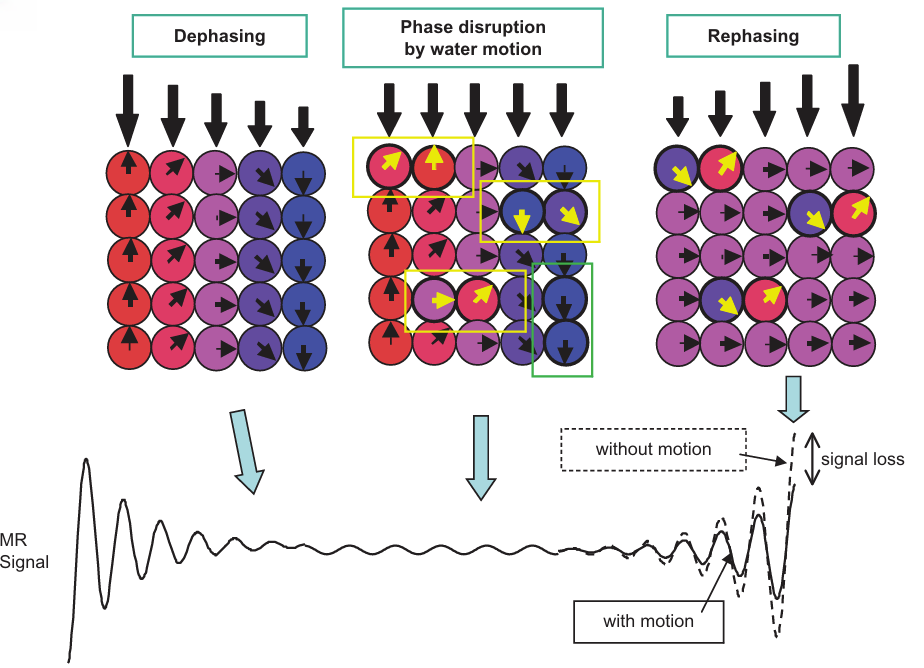
\includegraphics[width=0.7\textwidth]{Images/diffusion_2.png} % or use height= for vertical sizing
  \caption{Effect of dephasing and rephasing gradients on the phase of the spins. During dephasing and rephasing the magnetic field varies linearly with position (as indicated by the thick black arrows). The phase of the spins is indicated by the small arrows. Arrows in yellow indicate nuclei that diffuse in the gradient direction causing a net phase difference and consequently signal loss. In green, spins diffuse in the direction perpendicular to the gradient, causing no effect on the MR signal \cite{Mori20141}.}
  \label{fig:diffusion2}
\end{figure}



The values of ADC in a voxel reflect the underlying microstructure of the tissue. For example, in a voxel containing cerebrospinal fluid (CSF), the ADC is almost the same in all directions and fairly high, since diffusion is unrestricted. In contrast, within a WM voxel containing aligned fibre bundles, the ADC is significantly higher along the direction of the axons, and much lower in perpendicular directions due to restricted diffusion.

The typical spatial resolution of a diffusion-weighted MR image is on the order of a few millimeters, whereas the average displacement of water molecules during the measurement is between 1-20$\mu$m \cite{Mori20141}. As a result, the intensity of a diffusion-weighted image reflects the sum of many small contributions occuring at the microscopic scale.


The amount of signal loss is expressed as $\frac{S}{S_0}$, with $S_0$ the signal without diffusion weighting and S the measured signal, and it can be described by the equation:

\begin{equation}
\label{sig_att}
\frac{S}{S_0}=e^{-\gamma^2\cdot G^2\cdot\delta^2\cdot(\mathrm{\Delta}-\frac{\delta}{3})\cdot A D C}=e^{-b\cdot A D C}\
\end{equation}

where G and $\delta$ are the strength and length of the gradients. The signal loss increases with $\Delta$ and ADC, but also with G and $\delta$, as stronger or longer gradients determine more initial dephasing. G, $\Delta$, and $\delta$ are experimental parameters, while ADC is the quantity we want to estimate from the observed signal attenuation. The experimental parameters are combined into one parameter, the b-value, with units of $s/mm^{2}$. A higher b-value leads to greater signal attenuation.

\begin{figure}[h]
  \centering
  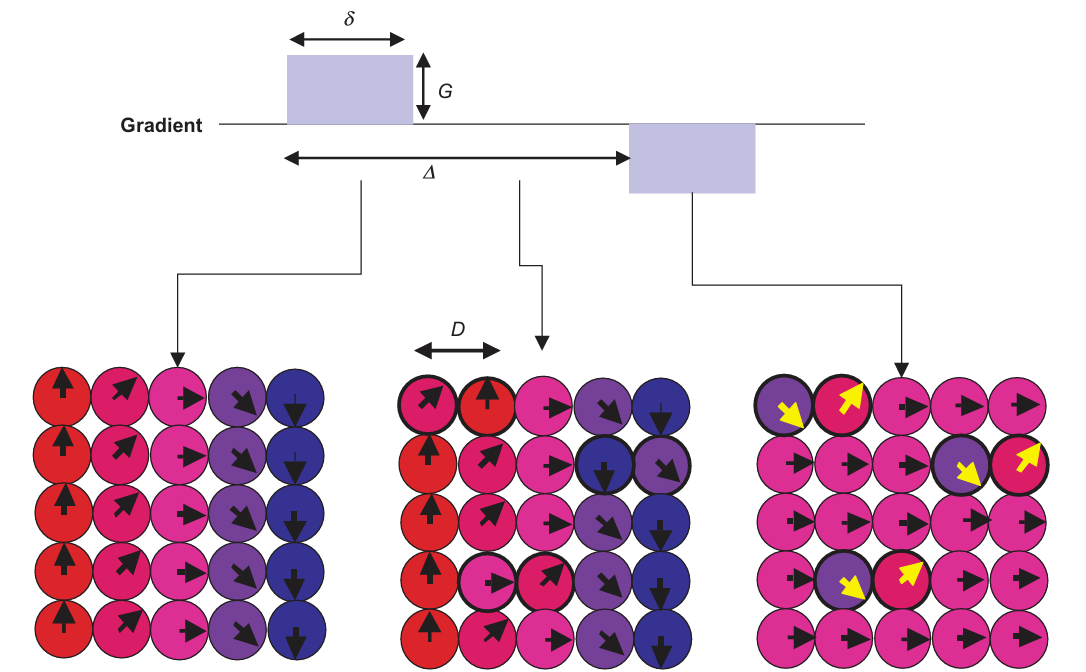
\includegraphics[width=0.7\textwidth]{Images/diffusion_1.png} % or use height= for vertical sizing
  \caption{Parameters of diffusion weighting ($\delta$, $G$, $\Delta$, D or ADC)\cite{Mori20142}.}
  \label{fig:diffusion1}
\end{figure}


 Taking the natural logarithm of the equation \eqref{sig_att} yields a linear relationship \cite{Mori20142}:

\begin{equation}
ln{(}\frac{S}{S_0})=-b\cdot ADC 
\end{equation}

This equation contains two unknowns: $S_0$ and ADC. Therefore, at least two measurements with different b-values are required to solve for ADC in a given gradient direction. In practice, more measurements are typically acquired to improve the signal-to-noise ratio (SNR), and a least squares fitting approach is used to estimate the parameters.

\section{Diffusion Tensor Imaging}
When diffusion is measured in complex, organized biological tissues such as WM, a single ADC value is insufficient to describe the behavior of water, as diffusion varies depending on the direction of measurement. To account for this anisotropy, a more sophisticated model called diffusion tensor imaging (DTI) was introduced \cite{ODonnell2011}. DTI models diffusion in each voxel as a 3x3 symmetric, positive-definite matrix known as the diffusion tensor, which captures the directional dependence of diffusion:

\[
D =
\begin{bmatrix}
D_{xx} & D_{xy} & D_{xz} \\
D_{xy} & D_{yy} & D_{yz} \\
D_{xz} & D_{yz} & D_{zz}
\end{bmatrix}
\]

The diffusion tensor contains six independent components, so at least six non-collinear, non-coplanar diffusion-weighted measurements are required, along with one unweighted reference image ($b$ = 0). Linear regression is then applied to the log-transformed diffusion signals to estimate the tensor components. In practice, more directions are often acquired to improve the robustness of the estimation using least squares fitting.

The diagonal elements of the tensor correspond to the diffusion coefficients along the three orthogonal axes, while the off-diagonal elements represent correlations between displacements along those axes. The tensor can be seen as a covariance matrix of molecular displacements \cite{Jones2013}, and it can be visualized as an ellipsoid. The surface of the ellipsoid represents the distance a water molecule, starting at the center, is likely to diffuse in each direction.
In the case of isotropic diffusion, where diffusion is equal in all directions, the ellipsoid becomes a sphere. In anisotropic diffusion, such as aligned WM fibres, diffusion is greater along one direction, and the ellipsoid becomes elongated along its principal axis. The principal axes of the ellipsoid are the eigenvectors of the diffusion tensor, and the lengths of these axes are proportional to the square roots of the eigenvalues ($\lambda_1$, $\lambda_2$, $\lambda_3$).

\begin{figure}[h]
  \centering
  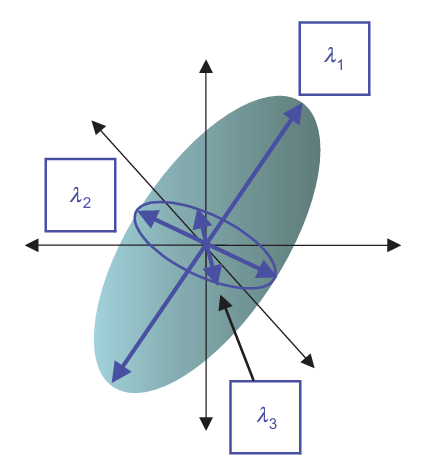
\includegraphics[width=0.6\textwidth]{Images/tensor.png} % or use height= for vertical sizing
  \caption{Diffusion tensor representation as an ellipsoid \cite{Mori20144}.}
  \label{fig:tensor}
\end{figure}

Several metrics can be derived from DTI. One widely used index is fractional anisotropy (FA), which quantifies the degree of anisotropy in a voxel:

\begin{equation}
\mathrm{FA} = \sqrt{\frac{3}{2}} \cdot \frac{\sqrt{(\lambda_1 - \bar{\lambda})^2 + (\lambda_2 - \bar{\lambda})^2 + (\lambda_3 - \bar{\lambda})^2}}{\sqrt{\lambda_1^2 + \lambda_2^2 + \lambda_3^2}}
\label{eq:FA}
\end{equation}

With $\bar{\lambda}$ the mean of the three eigenvalues. FA is defined as the normalized variance of the tensor's eigenvalues: it equals 0 in the case of isotropic diffusion and approaches 1 when diffusion is highly directional \cite{Jones2013}. FA quantifies the distance of the ellipsoid from a perfect sphere and is often interpreted as a measure of WM integrity.
Another commonly used metric is mean diffusivity (MD), calculated as the average of the tensor's eigenvalues.
MD provides a direction-independent measure of total diffusion within a voxel and is typically high in regions with free diffusion, such as cerebrospinal fluid \cite{LeBihan2001}.

As previously noted, diffusion MRI captures macroscopic signals that result from the aggregate effect of microscopic diffusion processes. This scaling difference between the physical phenomenon and what we can measure complicates the interpretation of voxel-wise metrics \cite{ODonnell2011}. At the same time, for microscopic phenomena to manifest at a larger scale, some degree of macroscopic structural coherence is required. This coherence influences which microstructural features can be detected using dMRI \cite{Mori20144}.

Information extracted from the diffusion tensor can also be used for tractography. Tractography is a method to estimate the trajectories of the fibre tracts in WM \cite{Lazar2010}. A common approach is streamline tractography, which works by successively stepping in the direction of the principal eigenvector (the direction of fastest diffusion) to reconstruct the tracts.

\section{Multi-shell Multi-tissue Constrained Spherical Deconvolution}

\subsection{DTI limitations}
One major limitation of DTI is its inability to resolve multiple fibre orientations within a single voxel, commonly referred to as crossing-fibres \cite{Seunarine2013}. Because DTI models diffusion using a second-order (rank-2) tensor, it can capture only one dominant diffusion direction per voxel. However, in many WM regions, the diffusion signal arises from more complex fibre geometries, such as crossing, kissing, or fanning fibres, which cannot be accurately represented by this simple model. In such cases, the diffusion tensor becomes not only inadequate but potentially misleading, compromising tractography results and undermining the interpretation of microstructural metrics like FA. A clear example of this limitation is the reported presence of low FA regions in deep white matter \cite{Mori20148}. These areas often contain two or more fibre populations oriented in different directions. Since DTI can only represent a single peak, it averages the signals from different directions, reducing the measured anisotropy and potentially leading to misinterpretation. An example can be seen in Figure~\ref{fig:crossing}.

\begin{figure}[h]
  \centering
  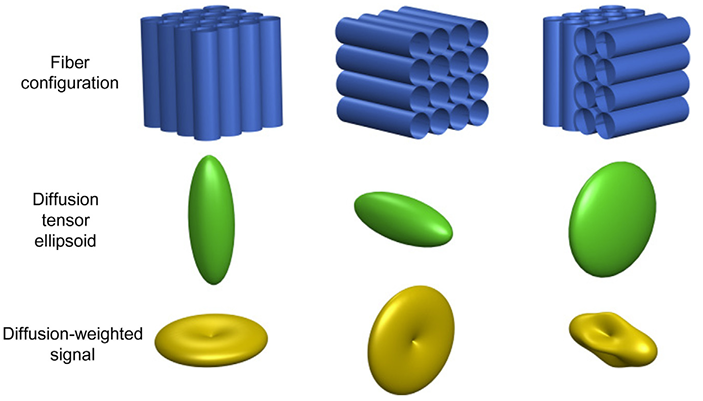
\includegraphics[width=0.7\textwidth]{Images/crossing.png} % or use height= for vertical sizing
  \caption{Example of how DTI can correctly recover the direction of fibres when only one fibre family is present (left and centre), but fails when two crossing families are present (right)\cite{Mori20148}.}
  \label{fig:crossing}
\end{figure}

\subsection{High angular resolution diffusion imaging}
This crossing fibres issue is highly relevant, as it is estimated that approximately 90\% of WM voxels contain more than one fibre population \cite{Jeurissen2013}. This limitation becomes critical in clinical applications such as neurosurgical planning, where tractography based on DTI may fail to identify important fibre bundles. Such false negatives could lead to incorrect conclusions about which brain regions are safe to operate on.

To address these limitations, methods are needed that can model multiple fibre populations within a voxel. To characterize the DW signal more exhaustively, High Angular Resolution Diffusion Imaging (HARDI) is employed \cite{Descoteaux2015}. HARDI is a data acquisition protocol that involves sampling the diffusion signal with many gradient directions uniformly distributed over a sphere for each b-value. Typically, the same set of directions is used across different b-values, forming multiple acquisition "shells".

This high angular sampling allows the angular features of the diffusion signal to be captured with finer resolution. Using multiple b-values further enhances the characterization of the signal, although it increases scan time. For DTI, the optimal b-value is generally around 1000 s/${mm}^{2}$, but for higher-order models that employ HARDI, the ideal b-value is less well-defined \cite{Mori20148}. Higher b-values improve the ability to resolve fibre orientations but also result in greater signal attenuation, reducing the SNR.
With HARDI data, it is possible to compute fibre orientation distribution functions (fODFs or simply ODFs). These functions describe the distribution of fibre orientations within a voxel. Defined over the unit sphere, the ODF assigns to each direction the probability of finding a fibre population aligned with it \cite{Seunarine2013}.

\subsection{Constrained Spherical Deconvolution}

A common method to recover the ODF from the diffusion signal is spherical deconvolution \cite{DellAcqua2019}. The core idea is to model the signal in each voxel as a combination of scaled and reoriented versions of a response function, the expected diffusion signal generated by a single, coherently oriented fibre population. The scaling is given by the fraction of fibres belonging to a certain family and the reorientation is needed to align the response with the fibre direction. The response function is typically derived by averaging the diffusion signal from voxels that are highly anisotropic and are presumed to contain only one dominant fibre orientation \cite{Tournier2007}. These signals are realigned to a common reference direction before averaging.

Mathematically, the total diffusion signal in a voxel is modeled as the convolution of this response function with the ODF, as shown in Figure~\ref{fig:convolution}.

\begin{figure}[h]
  \centering
  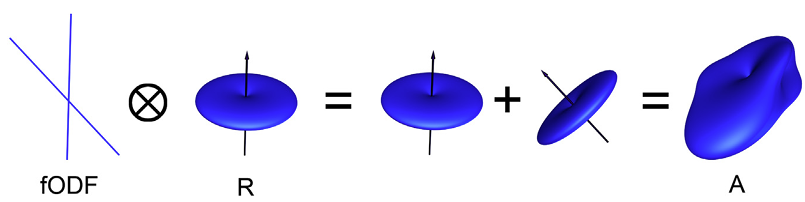
\includegraphics[width=0.7\textwidth]{Images/convolution.png} % or use height= for vertical sizing
  \caption{Convolution of the fODF with the response function R to obtain the measured diffusion-weighted signal A \cite{Seunarine2013}.}
  \label{fig:convolution}
\end{figure}

By inverting the operation, through spherical deconvolution, the ODF can be recovered. However, spherical deconvolution is an ill-posed problem, which could result in spurious peaks or negative values. To address this, regularization is applied, resulting in constrained spherical deconvolution (CSD). CSD imposes constraints to suppress physically implausible negative values and ensure a more reliable estimate of the ODF. For a single shell, CSD can be formulated as a constrained least squares problem \cite{Jeurissen2014}:

\begin{equation}
\hat{\boldsymbol{x}} = \arg\min_{\boldsymbol{x}} \frac{1}{2} \| C\boldsymbol{x} - \boldsymbol{d} \|_2^2 \quad \text{subject to} \quad A\boldsymbol{x} \geq \boldsymbol{0}
\label{eq:CSD}
\end{equation}

where $\boldsymbol{x}$ is the vector of coefficients of the ODF, $\boldsymbol{d}$ the vector of measured signal intensities, $C$ the matrix relating $\boldsymbol{x}$ to $\boldsymbol{d}$ by means of spherical deconvolution, and $A$ the matrix relating the ODF coefficients to their amplitudes.
CSD can effectively recover multiple fibre orientations within a voxel. An example of an ODF recovered using CSD in in Figure~\ref{fig:odf}. The peaks of the estimated ODF correspond to directions with the highest probability of having a fibre bundle, and the peak amplitudes are proportional to the underlying fibre density.
\\The use of ODFs has been shown to improve the reliability of tractography results when compared to traditional DTI methods \cite{Jeurissen2011}.

\begin{figure}[h]
  \centering
  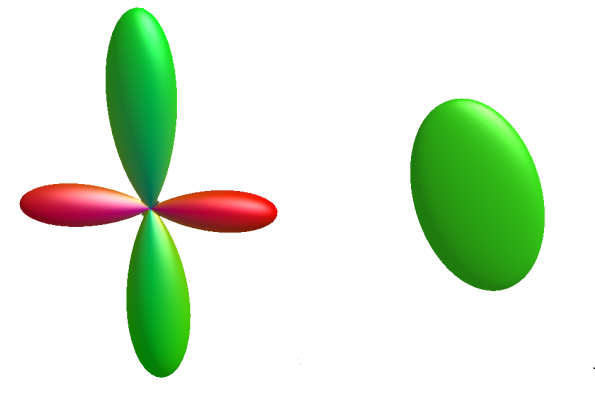
\includegraphics[width=0.5\textwidth]{Images/odf.png} % or use height= for vertical sizing
  \caption{An example of a fODF as recovered through CSD with the corresponding diffusion tensor next to it. The RGB color convention used to represent the directionality is red for right-left, blue for dorsal-ventral, and green for anterior-posterior.}
  \label{fig:odf}
\end{figure}

\subsection{Multi-shell multi-tissue CSD}
A more advanced model is Multi-Shell Multi-Tissue CSD (MSMT-CSD) \cite{Jeurissen2014}, which addresses limitations of single-tissue, single-shell CSD. Single-response models are accurate primarily in voxels containing pure WM, but can lead to overestimation of WM in voxels with mixed tissue types. MSMT-CSD addresses this by using multi-shell data and distinct response functions for different tissue types, typically WM, gray matter (GM), and cerebrospinal fluid (CSF). This approach not only estimates the fODF but also provides tissue-specific signal fractions within each voxel.
In MSMT-CSD, response functions are modeled using spherical harmonics (SH). The WM response function is assumed to be anisotropic and is modeled using a SH series of higher order, typically order 8 corresponding to 45 coefficients (Figure~\ref{fig:response}), while GM and CSF are modeled as isotropic and represented with SH series of order 0. Each response function is estimated separately for each b-value shell. 
Equation~\ref{eq:CSD} is extended to support m shells and n tissue types as follows:

\begin{equation}
\begin{bmatrix}
\hat{\boldsymbol{x}}_1 \\
\vdots \\
\hat{\boldsymbol{x}}_n
\end{bmatrix}
=
\arg\min_{\boldsymbol{x}}
\frac{1}{2}
\left\lVert
\begin{bmatrix}
{C}_{1,1} & \cdots & {C}_{1,n} \\
\vdots & \ddots & \vdots \\
{C}_{m,1} & \cdots & {C}_{m,n}
\end{bmatrix}
\begin{bmatrix}
\boldsymbol{x}_1 \\
\vdots \\
\boldsymbol{x}_n
\end{bmatrix}
-
\begin{bmatrix}
\boldsymbol{d}_1 \\
\vdots \\
\boldsymbol{d}_m
\end{bmatrix}
\right\rVert_2^2
\end{equation}

\[
\text{subject to } 
\begin{bmatrix}
{A}_1 & 0 & 0 \\
0 & \ddots & 0 \\
0 & 0 & {A}_n
\end{bmatrix}
\begin{bmatrix}
\mathbf{x}_1 \\
\vdots \\
\boldsymbol{x}_n
\end{bmatrix}
\geq 0
\]


Voxels dominated by a specific tissue type are selected to derive response functions. Originally, supervised approaches were used to define these voxels based on T1-weighted images and registration. More recently, unsupervised methods relying solely on diffusion data by analyzing signal decay and FA values have been developed and shown to improve accuracy \cite{Raffelt2016}.
\begin{figure}[h]
  \centering
  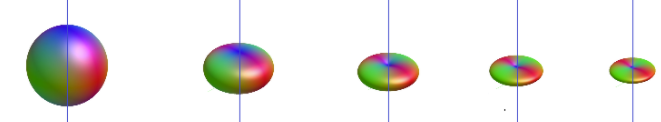
\includegraphics[width=0.5\textwidth]{Images/response.png} % or use height= for vertical sizing
  \caption{WM response function for 5 shells. With b=0 (no diffusion weighting) the response is isotropic, then with increasing b-value the signal is attenuated especially in the fibre direction.}
  \label{fig:response}
\end{figure}

MSMT-CSD is a powerful approach that can model multiple fibre orientations in each voxel with minimal assumptions, relying exclusively on diffusion data. It improves upon previous methods by using more data through incorporating multiple shells, and accounting for partial volume effects due to different tissue types.
However, limitations remain. The estimation of the response functions is largely heuristic, and the method relies on the assumption that a single average response function adequately represents all fibre populations across the brain. In reality, fibre characteristics such as configuration, cell size, and density may vary regionally \cite{Seunarine2013}. This is partially accounted for through ODF normalization \cite{Dhollander2021}, but some of the effects remain. Additionally, the standard three-tissue model does not account for atypical or pathological tissue types, which could lead to wrong results in brains affected by disease.

\section{Local Response Function estimation in Spherical Deconvolution}

To address the limitations of MT-CSD, a new method has been proposed: Local Response Function Estimation in Spherical Deconvolution (LoRE-SD). This approach eliminates the need for heuristic, global response function estimation by determining a voxel-wise response function directly from the data. As a result, the assumption that fibre populations generate the same signal across all brain regions is no longer required, making LoRE-SD more suitable for cases involving pathology or tissue types beyond the conventional WM, GM, and CSF classes.
\\In LoRE-SD, the response function in each voxel is modeled as a weighted sum of Gaussian basis functions, which are dependent on both the b-value ($b$) and the angle between the diffusion gradient direction and the fibre orientation ($\alpha$). These basis functions are parametrized by axial and radial diffusivity, and can be organized on a 10x10 grid representing all combinations of these two parameters, as shown in Figure~\ref{fig:grid}. Only the lower triangle of this grid is used, as the radial diffusivity must not exceed axial diffusivity.
Each Gaussian basis function is described as:

\begin{equation}
G_{\lambda_{\parallel}, \lambda_{\perp}}(b, \alpha) = 
e^{-b \lambda_{\perp}} \, 
e^{-b (\lambda_{\parallel} - \lambda_{\perp}) \cos^2 \alpha}
\end{equation}

Where $\lambda_{\parallel}$ and $\lambda_{\perp}$ are the axial and radial diffusivities.

\begin{figure}[h]
  \centering
  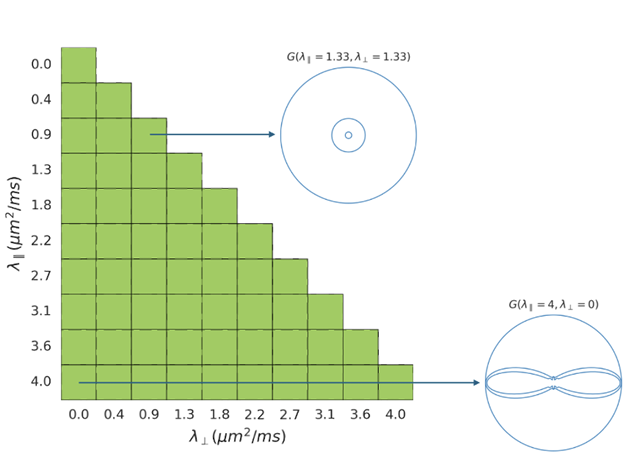
\includegraphics[width=0.7\textwidth]{Images/grid.png} % or use height= for vertical sizing
  \caption{Grid showing the Gaussian basis functions used to describe the response functions in LoRE-SD. $\lambda_{\parallel}$ and $\lambda_{\perp}$ are the axial and radial diffusivities.}
  \label{fig:grid}
\end{figure}

During optimization, in each voxel the method assigns a weight $f_{\lambda_\parallel, \lambda_\perp}$ to each basis function (Gaussian fractions). At each iteration, both the $f_{\lambda_\parallel, \lambda_\perp}$ and the SH coefficients of the ODF are estimated simultaneously for each voxel. The optimization problem is formulated as:

\begin{equation}
\min_{F, R} \quad \sum_{\ell \in \{0,2,\dots,\ell_{\max}\}} \left(S_\ell - \mathcal{N}_\ell R_\ell F_\ell^\top \right)^2 + \lambda \sum_{b,\ell>0} R_{b,\ell}^2
\end{equation}

Subject to:

\begin{equation}
F_0 = \frac{1}{\sqrt{4\pi}}
\end{equation}

\begin{equation}
Q F^\top \geq 0
\end{equation}

\begin{equation}
R = S_0 \sum_{\lambda_\parallel = 0}^{\lambda_\parallel^{(\max)}} \sum_{\lambda_\perp = \lambda_\parallel}^{\lambda_\perp^{(\max)}} f_{\lambda_\parallel, \lambda_\perp} G_{\lambda_\parallel, \lambda_\perp}
\quad \text{with} \quad 0 \leq f_{\lambda_\parallel, \lambda_\perp} \leq 1
\end{equation}

\begin{equation}
\sum_{\lambda_\parallel = 0}^{\lambda_\parallel^{(\max)}} \sum_{\lambda_\perp = \lambda_\parallel}^{\lambda_\perp^{(\max)}} f_{\lambda_\parallel, \lambda_\perp} = 1
\end{equation}

where $F$ represents the ODF, $R$ the response function and $S$ the diffusion signal. $\mathcal{N}_\ell$ is a normalization factor ($\frac{4\pi}{2\ell + 1}$) and $Q$ is a transformation matrix from spherical harmonics to spherical coordinates. $\lambda$ is a regularization parameter, usually $10^{-3}$ and $l$ represents the SH order. $l_{max}$ is usually set to  8.
A non-negativity constraint is imposed to the ODF (as for previous CSD methods) and the regularization term is used to promote isotropic response functions.
The ODFs generated by LoRE-SD are unit-normalized, meaning that, unlike the WM ODF resulting from MT-CSD, the amplitudes of their lobes do not inherently reflect fibre density. To assign meaningful magnitudes to the lobes, a scaling factor is required. This can be achieved using a contrast matrix, where each Gaussian basis function is assigned a weight (from 0 to 1) to emphasize or suppress specific basis functions. For example, a contrast matrix mimicking intra-axonal compartment can be obtained assigning high weights to basis functions with high axial and low radial diffusivity, with an exponential decay as radial diffusivity increases.
A contrast image is then computed for each voxel by taking the inner product between this contrast matrix and the basis function weights estimated in that voxel. This produces a scalar value per voxel, which is higher when the local signal aligns well with the response function described by the contrast matrix. An example for the described intra-axonal contrast is in Figure~\ref{fig:contrast}. These contrast images can then be used as voxel-wise scaling factors for the ODFs, assigning meaning to the amplitude of the lobes. Different contrast matrices can be designed depending on the tissue features of interest. 

\begin{figure}[h]
  \centering
  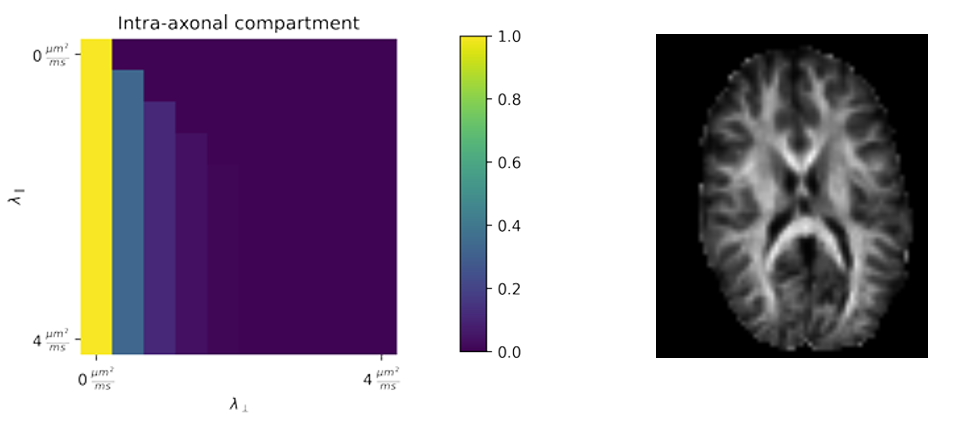
\includegraphics[width=0.7\textwidth]{Images/contrast.png} % or use height= for vertical sizing
  \caption{Contrast matrix used to define the intra-axonal contrast and example of the resulting contrast for one subject.}
  \label{fig:contrast}
\end{figure}

\section{Fixels}

DTI-derived metrics, such as FA, are widely used in voxel-based analysis (VBA) \cite{Liu2009}, where each voxel is assigned a scalar value and group-level statistical comparisons are performed. These studies can be cross-sectional (comparing different groups) or longitudinal (assessing changes over time, for example, due to disease progression). However, a key limitation of VBA is that it assigns a single scalar value per voxel, ignoring the fact that different fibre populations within a voxel may behave differently. This limitation reduces the biological specificity and interpretability of the results.
\\As mentioned, one of the main advantages of higher-order diffusion models like CSD is their ability to resolve complex fibre configurations, such as crossing fibres. By representing multiple fibre populations separately within a voxel, ODFs allow the extraction of fibre bundle-specific quantitative information, associating values not to the voxel but to the specific fibre orientations. In the previous sections, we described two methods for obtaining ODFs. In the first case (MT-CSD), the amplitude of the ODF lobes is intrinsically related to the apparent fibre density of the corresponding fibre population. In the second case (LoRE-SD), this relationship can be re-established by applying an appropriate scaling contrast, such as the intra-axonal compartment contrast.
\\To enable group-level analysis of this fibre-specific information, an important step is the extraction of fixels \cite{Raffelt2017}. A fixel is defined as a single fibre population within a voxel. Fixels are extracted by identifying the direction of each ODF lobe peak, with only those above a certain amplitude threshold retained to reduce the inclusion of spurious or noisy peaks. Each fixel is represented as a line segment passing through the center of the voxel, as the actual position of the fibre family within the voxel cannot be known. The information is in the directionality, while the length has no meaning. A single voxel can contain multiple fixels, or none at all, depending on the underlying fibre structure. An example of ODFs and the extracted fixels is shown in Figure~\ref{fig:fixel}. Taking inspiration from VBA, a Fixel-Based Analysis (FBA) can be performed, assigning metrics to individual fixels rather than entire voxels \cite{Dhollander2021}. These fixel-wise metrics can reflect fibre-specific properties, potentially tied to only specific microstructural compartments within a voxel. However, working with fixels introduces new challenges, including registration, fixel correspondence across subjects, and statistical inference. These topics, along with the detailed FBA pipeline, will be discussed in the next section.

\begin{figure}[h]
  \centering
  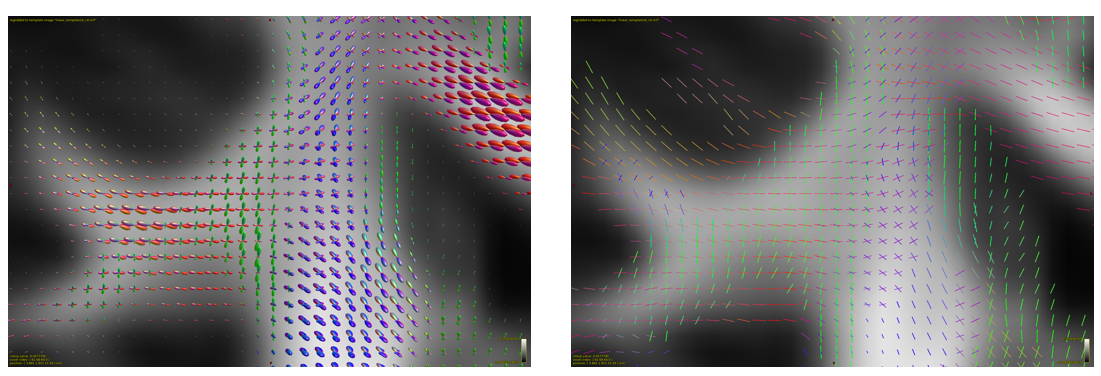
\includegraphics[width=0.8\textwidth]{Images/fixel.png} % or use height= for vertical sizing
  \caption{Left: WM ODFs found with MSMT-CSD. Right: corresponding fixels. In both images the colors represent the directionality. The RGB color convention used is red for right-left, blue for dorsal-ventral, and green for anterior-posterior.}
  \label{fig:fixel}
\end{figure}

\section{Fixel Based Analysis}
\label{sec:fba}
Below, we outline the metrics used in FBA and the standard pipeline that starts from WM ODFs derived from MT-CSD, before describing the changes introduced by LoRE-SD in a later section.

\subsection{Apparent Fibre Density}
The first fixel-wise metric derived from a WM ODF is Apparent Fibre Density (AFD) \cite{Raffelt2012}. This metric is calculated by numerically integrating the amplitude of the ODF lobe along a given direction using dense angular sampling \cite{Smith2013}. The amplitude of the ODF in a specific orientation is proportional to the DW signal perpendicular to that orientation, which in turn reflects the intra-axonal water fraction, or in other words, the density of the fibres.
Since ODF amplitude is influenced by both the underlying fibre population and the response function used during deconvolution, in a study it is critical to use a common response function across all subjects. This ensures consistent scaling of the ODFs, making inter-subject comparisons meaningful. A typical strategy involves averaging the response functions across all subjects to obtain a study-specific response function.
AFD is influenced both by axon count and axon diameter \cite{Dhollander2021} and it can be interpreted as a the fibre bundle's capacity to transfer information \cite{Raffelt2012}. However, AFD is also affected by the presence and the changes of other fibre populations or other tissue compartments in the same voxel, which can confound the interpretation.

\subsection{Intensity normalization and bias field correction}
An essential step in MT-CSD-based FBA is intensity normalization, which aims to make AFD values comparable across subjects \cite{Raffelt17}. This step ensures that the total diffusion signal, summed across all tissue compartments, remains approximately constant throughout the brain. This assumption helps correct for bias fields and for the fact that a single response function may not be representative of the whole brain. After normalization, the WM, GM, and CSF ODFs are scaled to comparable units.

\subsection{Template Construction and Registration}
Group analysis begins with the creation of a study-specific template. This is typically built using ODFs from a representative subset of subjects (excluding anatomical outliers). After initialization with an initial average image, the construction follows an iterative process:

\begin{enumerate}
    \item Registration of each subject to the template.
    \item Template update as the mean of the registered images.
\end{enumerate}

A possible approach is using rigid registration for the first iterations, then affine, and finally nonlinear.
Higher order information contained in the ODFs has been shown to improve the results of registration, compared to FA- or T1-based methods \cite{Raffelt2011}. At each iteration, each ODF is spatially transformed, interpolated and then reoriented using local angular transformations. This last step ensures that the orientation information remains anatomically correct with respect to the new spatial configuration.
ODF reorientation is performed using a point spread function (PSF) model: the ODF is approximated as a sum of PSFs, each of which is transformed individually. The transformed PSFs are then summed to obtain the final reoriented ODF \cite{Raffelt12}. A diffeomorphic transformation is used to ensure that the Jacobian determinant remains positive, a necessary condition for proper ODF reorientation.

Once the ODF template is obtained, ODF-guided registration is used to move subjects data to the common space, which results is the nonlinear warps that will be used to extract the next metric. The transformation is applied, but roerientation is delayed to a later step. This means that the transformed ODF images are anatomically-broken.

\subsection{Fixel Extraction and Correspondence}
A fixel mask is generated by segmenting the template ODFs. Only lobes above a certain amplitude threshold, indicative of consistent fibre presence across subjects, are retained. The amplitudes are lower were subject ODFs align less well, for example at the GM/WM interface where the inter-subject variation is high and registration is imperfect.

Then for each subject:

\begin{enumerate}
    \item Fixels are extracted from their WM ODFs in template space.
    \item Fixels are reoriented using the nonlinear warp.
    \item AFD values are computed by integrating the amplitude of each valid lobe and are assigned to the corresponding fixel.
\end{enumerate}

Fixel correspondence between subject and template is established by searching, within each voxel, for matching fixels in the template (within an angular threshold). If no match is found, the AFD value is set to zero for that fixel in that subject.

\subsection{Fibre-Cross Section}
An additional metric that can be derived directly from the spatial warp fields is the Fibre Cross-Section (FC) \cite{Raffelt2017}. The nonlinear warp used to register a subject to the template describes the local volume change, quantified by the determinant of the Jacobian matrix ($det( J)$). When analyzing WM fibres, only changes perpendicular to the fibre orientation are biologically meaningful, as they reflect alterations in the number of axons across a bundle's cross-section.

FC measures these perpendicular volume changes, providing complementary information to AFD and is defined as:
\begin{equation}
FC_f = \frac{det( J)}{\lVert J\hat{\boldsymbol v}_f\rVert}
\end{equation}

where the component in the direction of the fixel f (described by the unit vector $\hat{\boldsymbol v}_f$) is factored out from the total volume change.
This is a relative metric, as it describes the volume change relative to the template. This means that it can only be compared across subjects in the same study and only in corresponding brain regions.
While AFD reflects microstructural changes (the axonal density), FC captures macrostructural changes (the bundle size).

An additional metric can be derived as the fixel-wise product of AFD and FC, known as Fibre Density and Cross-section (FDC) \cite{Raffelt2017}. This metric provides a more comprehensive measure that accounts for both microscopic and macroscopic changes in WM. FDC can thus be interpreted as reflecting the total intra-axonal volume, combining information about the number of axons and their spatial distribution in the brain.
However, interpreting these three metrics is not always straightforward and must be contextualized within the underlying pathology. For instance, in a disease process that initially causes axonal loss, a reduction in AFD might be expected in the affected regions. But if atrophy occurs later, reducing the cross-sectional area of the tract, the remaining axons may become more densely packed, potentially leading to an unexpected increase in AFD. In such a scenario, FC would be reduced, and FDC might remain unchanged, emphasizing the importance of considering all three metrics together to accurately characterize pathological changes. A graphical example of this situation is in Figure~\ref{fig:atrophy}.
Finally, it is important to note that the separation between AFD and FC is not always clear-cut in practice \cite{Dhollander2021}. Due to the limitations of non-rigid image registration, part of an effect that should be attributed to FC may instead be attributed to AFD, and vice versa. This ambiguity is particularly pronounced in small or thin structures, and means that AFD and FC should not be directly compared in terms of effect size. Therefore, FDC is often a more reliable metric, as it incorporates both effects.\\

\begin{figure}[h]
  \centering
  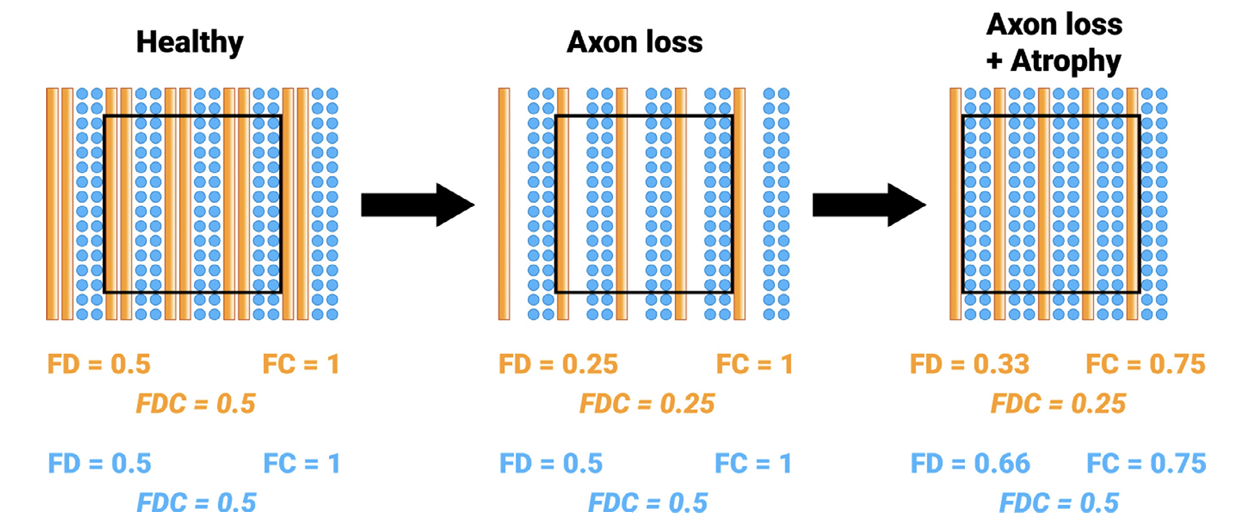
\includegraphics[width=0.8\textwidth]{Images/atrophy.png} % or use height= for vertical sizing
  \caption{Example of how the three metrics need to be considered together and that metrics related to one fibre family are influenced by the other components in the same voxel. By just considering AFD (FD) for the blue fibre family, one may conclude that the disease leads to an increase of the number of axons. But this is due to the atrophy as it can be inferred by the decrease of FC and the constant FDC. Additionally, even though AFD and FC change for the blue family, the disease didn't have a direct effect on the blue axons. The change is due to the blue fibres sharing the voxel with the affected orange fibres \cite{Dhollander2021}.}
  \label{fig:atrophy}
\end{figure}

In VBA, once anatomical correspondence between subjects is established through registration, the next steps are smoothing the images, performing voxel-wise statistical testing, and assigning p-values based on statistical inference \cite{Raffelt2015}. These steps must be adapted for FBA, as fixels in neighboring voxels may belong to different fibre populations and comparisons need to be fixel-wise.

\subsection{Smoothing Using Structural Connectivity}
In VBA, smoothing of the metrics is typically applied using a Gaussian kernel centered on each voxel, averaging across neighboring voxels to improve SNR, reduce registration errors, and increase robustness. However, this method is not directly applicable to fixels because adjacent voxels may contain unrelated fibre populations. Instead, FBA requires a smoothing strategy that respects WM tract architecture. To achieve this, a whole-brain probabilistic tractography is generated on the ODF template. This is used to define structural connectivity between all fixels, resulting in a fixel-fixel connectivity matrix \cite{Raffelt2015}. This is a sparse matrix where each element $c_{ij}$ is the proportion of streamlines passing through fixel i that are also passing through fixel j. These values are combined with a Gaussian kernel centered at the fixel of interest to weight the contribution of structurally connected fixels during smoothing. This ensures that only anatomically connected fixels influence one another.

\subsection{Statistical Testing and Inference in FBA}

As in VBA, statistical inference in FBA must address the problem of multiple comparisons. A popular solution for VBA relies on the idea that true positives will form spatially coherent clusters, as the underlying anatomy or pathology is shared among them. This is known as cluster-based inference \cite{Winkler2014}. Threshold-Free Cluster Enhancement (TFCE) avoids choosing an arbitrary threshold for forming clusters by integrating across all thresholds, resulting in an enhanced test statistic that reflects both the original test statistic values and the spatial extent of the clusters.

An approach inspired by TFCE but adapted for FBA is connectivity-based fixel enhancement (CFE) \cite{Raffelt2015}. CFE uses the fixel-fixel connectivity matrix to define clusters of structurally connected fixels and enhance the statistical power. The connectivity information is used to weight contributions from neighboring fixels when computing the enhanced test-statistic: fixels more structurally connected to the one of interest contribute more strongly. The goal is to recover statistical power lost due to correction for multiple comparisons by assuming that changes in one fixel are likely to co-occur along structurally related WM pathways.

Statistical hypotheses in fixel-based analysis are typically framed within a general linear model (GLM). The GLM allows modeling each fixel-wise metric (AFD, FC, FDC) as a linear combination of explanatory variables (e.g., group, age), encoded in a design matrix. Model parameters are estimated, and statistical tests (t-tests) are performed at each fixel to assess the effects of interest.

Permutation testing is the preferred method for inference, as it reduces the number of assumptions. The only requirement is exchangeability under the null hypothesis \cite{Winkler2014}. This involves randomly permuting the data (e.g., reassigning group labels) and recalculating the test statistic for each permutation. The p-value is the proportion of permutations with a test statistic as extreme or more extreme than the observed one, which quantifies evidence against the null hypothesis.

To address the issue of multiple comparisons, permutation testing is also used to compute family-wise error (FWE) corrected p-values. This is done by recording the maximum test statistic across all fixels for each permutation, creating a distribution of maximal values. The FWE-corrected p-value for each fixel is then the proportion of permutations in which the maximum statistic exceeds the observed one. This approach is compatible with CFE: at each permutation the maximum cluster-enhanced test statistic is recorded.\\
Finally, statistically significant fixels can be identified as those with a FWE-corrected p-value below 5\%.

\section{FBA and LoRE-SD}
FBA can be extended to ODFs derived from LoRE-SD. Unlike MT-CSD ODFs, which require intensity normalization across subjects, LoRE-SD ODFs are unit-normalized by design. The first step is selecting a specific contrast which assigns a scaling factor to each ODF.

In MT-CSD, ODF lobe amplitudes are directly influenced by the response functions, with the WM response function acting as a "unit," thus enabling direct comparison across subjects. In LoRE-SD, however, the lobe amplitudes depend on the chosen contrast via the response function representation. Comparability across subjects is ensured by using the same contrast matrix for all. The metric resulting from integrating the ODF lobe, analogous to AFD, will reflect the chosen contrast. FC and FDC can be computed using the deformation fields (warps) obtained during registration to the population template, following the same steps as in the MT-CSD-based pipeline.

The most computationally intensive step of the FBA pipeline is creating the study-specific template via non-linear ODF registration. If different contrasts are applied to scale the ODFs, they only differ by a multiplicative constant at each voxel. This suggests that a template constructed with one contrast (e.g., intra-axonal) could potentially be reused with ODFs scaled using other contrasts. This is because the deformation fields (warps) represent spatial transformations, which should ideally be contrast-independent. In practice, however, the iterative nature of registration and template construction means that using a different contrast (or even re-registering with the same contrast) results in slightly different warps. As long as these discrepancies are small, the FBA pipeline compensates for them via smoothing, which is guided by the fixel-fixel connectivity matrix.\\ While it's possible to build the template from unscaled (unit-normalized) ODFs, this may be suboptimal, as registration would be driven purely by directional information. Scaled ODFs incorporate amplitude information, which can improve registration accuracy, particularly since the same contrast representation is used across subjects, making lobe amplitudes more or less consistent in corresponding brain regions.

So, using the same warps for differently scaled ODFs may be acceptable, with the main consequence being a change in the extracted AFD-like values. FC remains unchanged, as it depends solely on the warp fields. Consequently, the fixel correspondence between subject and template is preserved, and only the amplitude (integrated lobe value) associated with each fixel will vary. Employing multiple contrasts to scale the ODFs could be useful, as extracted metrics from each one could give us unique insights. As a result, statistical testing on AFD or FDC may be different depending on the contrast used to scale the ODFs. While FC remains unaffected, differences in amplitude scaling may influence effect sizes and statistical significance for the other two metrics.

\section{Chemobrain and Diffusion MRI}

Several studies have used DTI to investigate WM changes associated with chemotherapy, particularly on breast cancer patients. Matsos et al. \cite{Matsos2017} reported that chemotherapy-treated patients performed worse than healthy controls in tests of attention and psychomotor speed. These deficits were accompanied by reduced FA in frontal, occipital, and parietal WM tracts. Similarly, Deprez et al. \cite{Deprez2011} performed a study on breast cancer patients and observed decreased FA in frontal and temporal WM regions, along with increased MD in frontal tracts. Additionally, they found that lower FA values correlated with poorer cognitive test performance, particularly in the superior longitudinal fasciculus and inferior longitudinal fasciculus.

Longitudinal studies have offered additional insights. Chen et al. \cite{Chen2020} investigated older breast cancer patients ($\geq$60 years) before and within one month after chemotherapy. While no significant changes in FA were detected, they observed increased MD and radial diffusivity in the genu of the corpus callosum post-treatment. Another study by Koppelmans et al. \cite{Koppelmans2014} focused on long-term effects and found no significant differences in DTI metrics between healthy controls and breast cancer survivors. However, they did identify a negative correlation between time since treatment and WM integrity, with lower FA and higher MD over time.
Deprez et al. \cite{Deprez2012} conducted a longitudinal assessment of cognitive performance and DTI metrics again on breast cancer patients. Patients showed a decline in cognitive test scores 3-4 months after chemotherapy, along with decreased FA in frontal, parietal, and occipital WM tracts. These FA reductions correlated with performance declines, suggesting a link between treatment-induced WM changes and cognitive impairment. The observed microstructural alterations may reflect axonal injury or demyelination, both of which impact WM diffusivity.

FBA has also been employed to study the impact of chemotherapy. Schroyen et al. \cite{Schroyen2021} compared chemotherapy-treated breast cancer patients, non-chemotherapy patients, and healthy controls but found no significant group differences in fixel-wise metrics, possibly due to limited sample size. However, they identified a negative association between log-transformed FC (log-FC) in the corpus callosum and glial cell overexpression, indicating possible neuroinflammation. The corpus callosum, being densely packed with axons and highly vascularized, may be especially vulnerable to chemotherapy-induced damage.

\section{Aim of the Thesis}

The aim of this thesis is to apply the LoRE-SD method within a FBA framework and to compare the results with those obtained using the standard approach based on WM ODFs derived from MT-CSD. This will allow us to assess whether LoRE-SD is suitable for integration into the FBA pipeline. Furthermore, the flexibility introduced by LoRE-SD's scaling may enable the extraction of additional and potentially more meaningful microstructural information than with MT-CSD alone. Since FBA results depend on both the ODFs and the applied modulation, we will investigate whether different scaling strategies affect the significance and the distribution of the detected effects.
\\This analysis will be carried out in the context of a group study involving breast cancer patients undergoing chemotherapy, patients not receiving chemotherapy, and a control group of healthy subjects. An additional objective is to investigate whether chemotherapy induces detectable changes in WM. We hypothesize that significant group differences in fixel-wise metrics may be found, particularly in WM regions involved in memory and cognitive functions. Such differences may reflect disruption of WM integrity, potentially underlying the cognitive decline observed in some patients.